\section{Diverses}
    \subsection{Von $G(s)$ zur DGL}
    	\begin{multicols}{2}
    		\begin{itemize}
  				\item $G(s)$ als Bruch aufschreiben.
  				\item Zähler = Eingang ($u$) \quad Nenner = Ausgang ($y$)
  				\item $j\omega = \dot{y} \quad (j\omega)^2 = \ddot{y} \quad \ldots $
  				\item Gleiches gillt für den Zähler mit u!
			\end{itemize}
			\columnbreak
			\textbf{Beispiel:} $G(s) = \frac{K(j \omega T + 1)}{(j\omega)^2 T_N + j \omega Tn(1+K_R) + K_R}$ \\			
			\textbf{DGL:} $T_N \ddot{y} + T_N(1+K_R) \dot{y} + K_R y = K(T \dot{u} + u)$
    	\end{multicols}    	
    
    \subsection{Zeigerdiagramme}
    Soll zu einem Gegebenen Blockschaldbild (oder einer gegebenen Funktion) das Zeigerdiagramm erstellt 
    werden werden die \textbf{Beträge} der Elemente \textbf{multipliziert},
    die \textbf{Winkel} ($arg()$) \textbf{addiert}. Die Werte für die einzelnen Elemente sind der Tabelle in 1. LTI-Grundglieder zu entnehmen. 


	\subsection{Graphisch Phasen-/Verstärkungsreserve}
		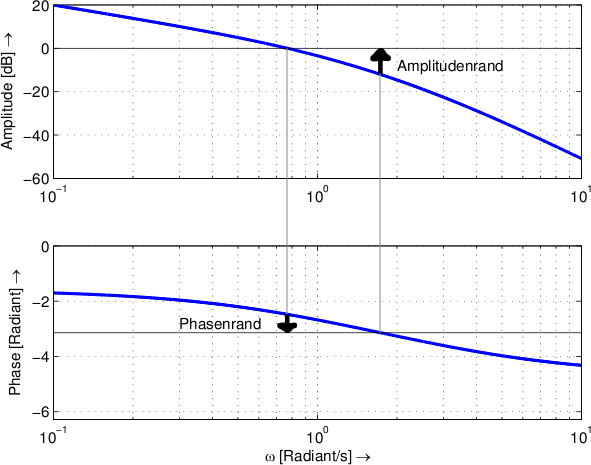
\includegraphics[width=7cm]{./images/bode-stabilitaet.png} \\
		Phasen-/Verstärkungsreserve = Phasen-/Amplitudenrand

